% !Mode:: "TeX:UTF-8"

\chapter{代码中间表示提取与分析特征提取}

%%%%%%%%%%%%%%%%%%%%%%%%%%%%%%%%%%%%%%%%%%%%%%%%%%%%%%%%%%%%%%%%%%%%%%%%%%%%%%%
\section{引言}

\section{基于clang的抽象语法树生成方法}
抽象语法树(Abstracted Syntax Tree,AST)是一种用来表现编程语言构造的树状
结构,它把代码的语法结构以树形的方式进行了抽象化描述。在这个树形结构中,每一
个节点都对应着代码中的某个元素,比如变量声明、语句或者是表达式等。从这棵树的
根节点出发,代码逐步被拆解成更小的部分,直到最终到达叶节点,这些叶节点代表了
代码中最基本的元素,如操作符或变量等。在这棵树中,节点之间的连接仅表明了它们
之间的层级关系,即父节点与子节点的关系。通过这样的结构,AST 能够清晰地展示出
代码的层次和结构,为编译器或其他工具分析和处理代码提供便利。


Clang 是由苹果公司发起的支持 C、C++、Objective-C 和 Objective-C++语言的编译
器前端,负责对代码进行词法分析、语法分析和语义分析,对程序代码的分析和理解至
关重要[7]。词法分析通过识别 Token 将程序代码分解成基本单元。语法分析在此基础上
识别程序的语法结构,构造抽象语法树。语义分析消除语义模糊,生成属性信息,让计
算机生成目标代码。libclang 是 Clang 编译器的一个重要组成部分,提供了一套用于解
析源代码的程序接口。这些程序接口允许开发者在自己的项目中使用 Clang 的强大语言
解析和代码分析功能[8]。为提取代码中的调用和依赖关系,本课题使用了 libclang 生成
AST 的能力,为后续进一步分析提供基础。


如图 2-2 所示,举例说明 clang 的使用。这里定义了一个简单的 C 语言文件,定义
了两个函数和一个全局变量,主函数用于计算两个数的和。
\begin{figure}[h]
\centering
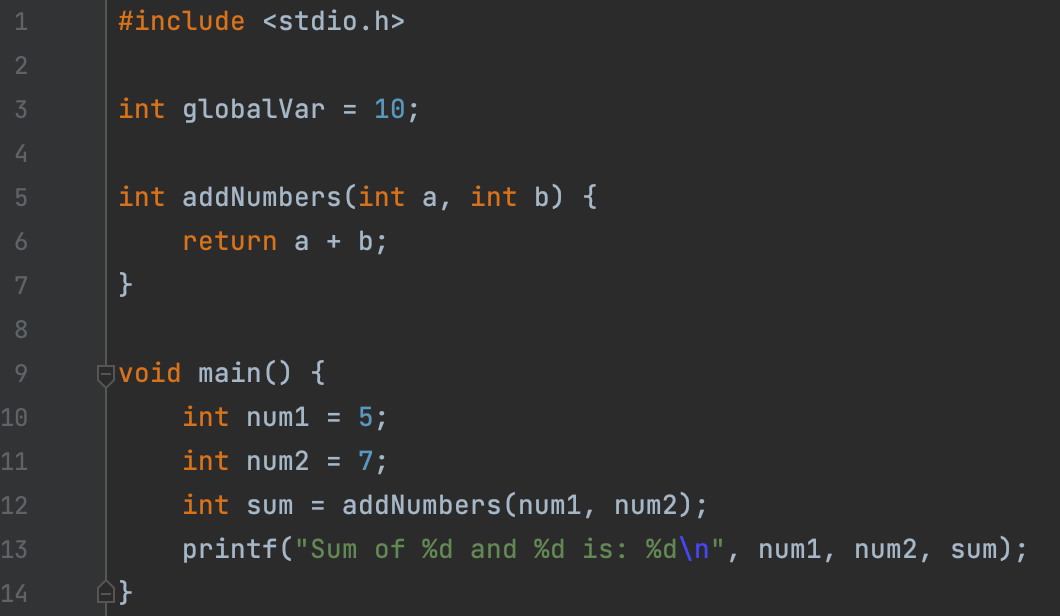
\includegraphics[width = 0.6\textwidth]{代码示例}
\caption{示例代码}
\end{figure}

这段代码由 Clang 解析生成抽象语法树后,得到的树结构如下图 2-3 所示。
\begin{figure}[h]
\centering
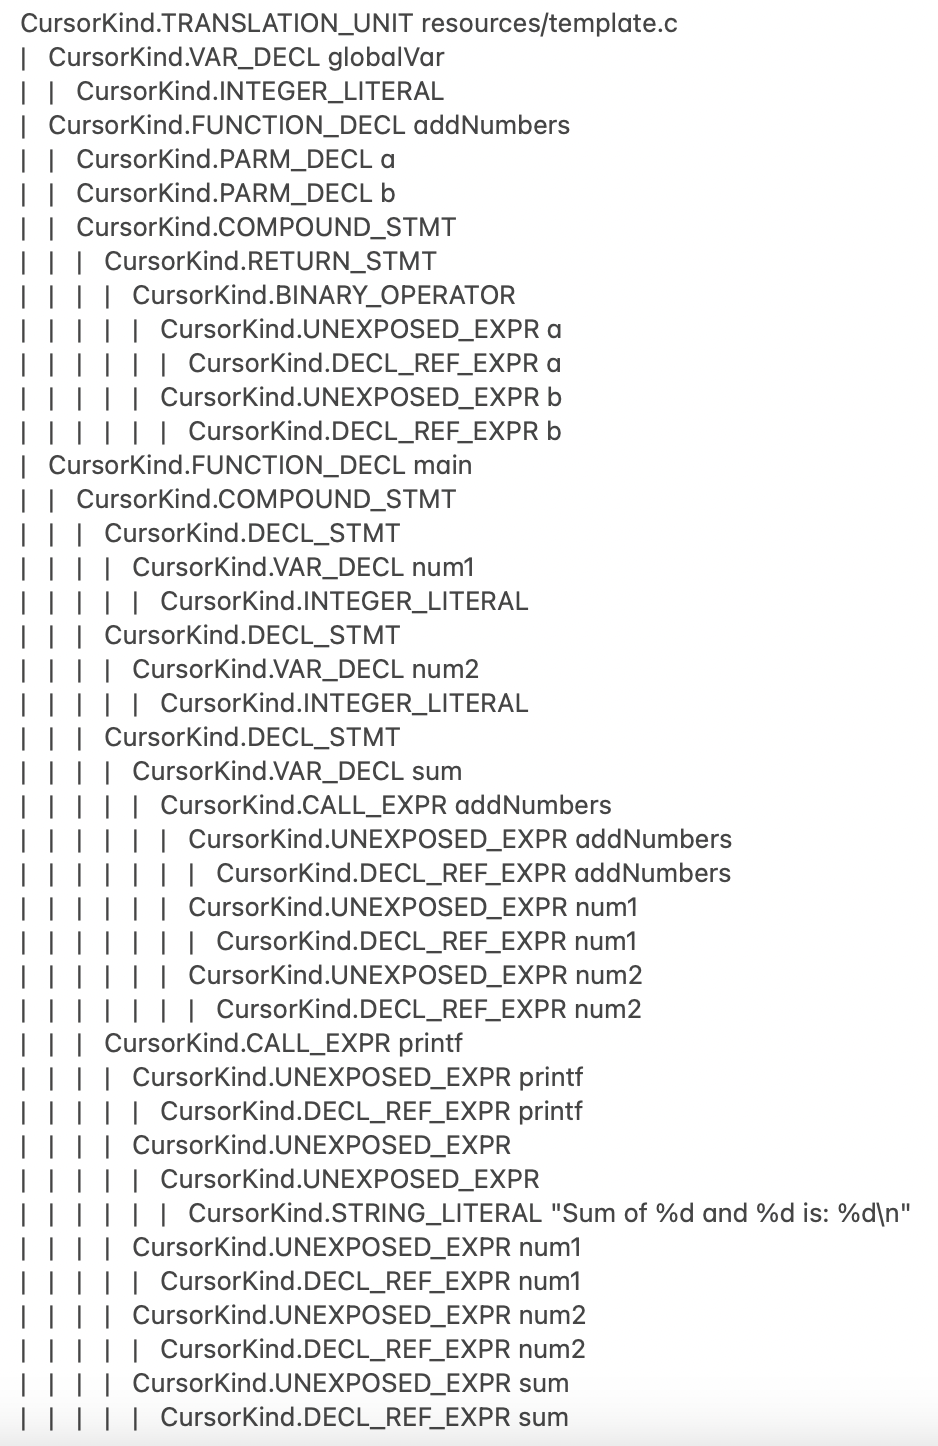
\includegraphics[width = 0.6\textwidth]{ast示例}
\caption{示例代码对应的抽象语法树结构}
\end{figure}

在 libclang 解析得到的抽象语法树中,游标(cursor)是一个核心概念,它作为一个
指针或引用存在,每个 cursor 都与 AST 中的一个特定节点相对应,表示了源代码中的
一个结构元素。通过操作 cursor,可以遍历整个 AST,访问和分析代码中的各种元素,
如获取变量的类型、函数的参数列表、类的成员等。libclang 提供了一系列 API 函数来
操作 cursor,例如:遍历 AST 中的 cursor、获取 cursor 的类型(如是否为方法定义、变
量定义、变量引用等)、获取 cursor 所代表的源代码元素的名称、类型、位置等信息、
获取 cursor 的父节点或子节点等。这里我们通过操作游标,遍历 AST,获取整个 AST
的结构。


Clang 定义了一套节点类型标识。AST 的顶层节点类型是Translation\_Unit标签,表
示一个翻译单元,对 AST 树的遍历,实际上就是遍历整个 Translation\_Unit。Function\_Decl
指的是函数定义,在 clang 中是不区分函数声明和函数定义的,统一用 Function\_Decl
来标识,两个区分主要看是否有函数体,在 libclang 中提供了程序接口共我们调用判断。
Parm\_Decl 是参数节点,上面的例子中,函数 addNumbers 有两个参数 a 和 b。
CompoundStmt 代表大括号,函数实现、struct、enum、for 的 body 等一般用此标签包起
来。DeclStmt 是定义语句,里边可能有 VarDecl 等类型的定义,VarDecl 是对变量的定
义。CallExpr 标签表示函数调用 Expr,子节点有调用的参数列表。ReturnStmt 表示返回
语句。






\section{方法调用链提取与分析}
代码项目中的方法之间的调用关系是本课题中的分析基础。在使用 Clang 提取到
AST 后,遍历整棵树来提取方法之间的调用关系。这部分我们重点关注 AST 上的方法
节点,以及节点内部的调用节点。


对 AST 的遍历主要分为两次,第一次遍历获取所有的方法定义。首先提取所有的
FUNCTION\_DECL 节点,它表示了对方法的定义,在该节点中可提取方法签名。在
FUNCTION\_DECL 节点下,提取子节点 PARM\_DECL,该节点表示方法的参数列表,
在该节点中可提取参数名称和参数类型等参数相关信息。然后提取 FUNCTION\_DECL
节点的子节点 VarDecl,该节点表示在该方法内定义的局部变量。在对方法进行分析时,
我们本身不关心方法的内部实现,但是由于在 C/c++语言中,存在局部变量可以和全局
变量重名的情况,在这里提取方法内定义的局部变量,方便后续在提取全局变量时,对
变量进行作用域的判断。除此之外,还需提取整个方法的 token 序列,所在文件以及作
用域。


第二次遍历的主要目的是提取方法之间的调用关系。提取 FUNCTION_DECL 节点
的子节点 CALL_EXPR,该节点标签表示的是调用语句,可提取调用的方法名。注意,
由于主要分析该项目中由开发者定义的方法之间的依赖关系,所以对于一些标准库方法
的调用选择忽略,不进行提取。具体的计算流程如算法 2-1 所示。

分析结束后,将会获得每个方法的方法调用链,对应于一个方法摘要表,包括项目
代码中所有的方法和方法之间的调用关系,除此之外还包括方法的参数表、方法主体和
所在文件等其他信息。

\section{全局变量定义-使用链提取与分析}

全局变量定义-引用链的提取和方法的定义和调用提取是类似的。对 AST 的遍历主
要也分为两次。具体流程如图第一次遍历获取所有的方法定义。首先提取所有的
VAR_DECL 节点,它表示了对变量的定义,然后提取节点中的变量名和变量类型。注
意由于在 AST 中的节点标签中无法区分变量是否是全局的,所以这里根据节点在 AST
中的深度来判断是否是全局变量,并且在变量名前加上针对该项目文件的绝对路径,来
保证变量名的唯一性。在确定其为全局变量后,还需进一步提取该变量的作用域。在
C/c++语言中,可将变量和方法声明为 static 的,意味着该变量或该方法只能在其所在文
件内使用,而不是全局可用,所以需要对其作用域进行判断。一次遍历提取到的结果是
一个全局变量表,这里使用哈希表 Map<Name, globalVar>的数据结构进行存储,方便对
全局变量进行查找。

第二次遍历的主要目的是提取全局变量的引用点。在方法节点子树中搜索
DECL\_REF\_EXPR 节点,它表示对变量的引用,这里首先判断被引用的变量是否是局部
变量,根据函数摘要表中该函数的记录可以判断,如果是则直接返回,如果不是,则证
明使用的是全局变量,这里首先对该变量名在哈希表中进行查找,如果查找到了,说明
是在该文件中定义的全局变量,以节省检索时长,同时能够保证如果是 static 的全局变
量的准确性。如果没有查找到,则说明引用了别的文件中定义的全局函数,则就在哈希
表中进行遍历查找,记录该全局变量被引用的方法。具体计算流程如图 2-3 所示。

\begin{figure}[h]
\centering
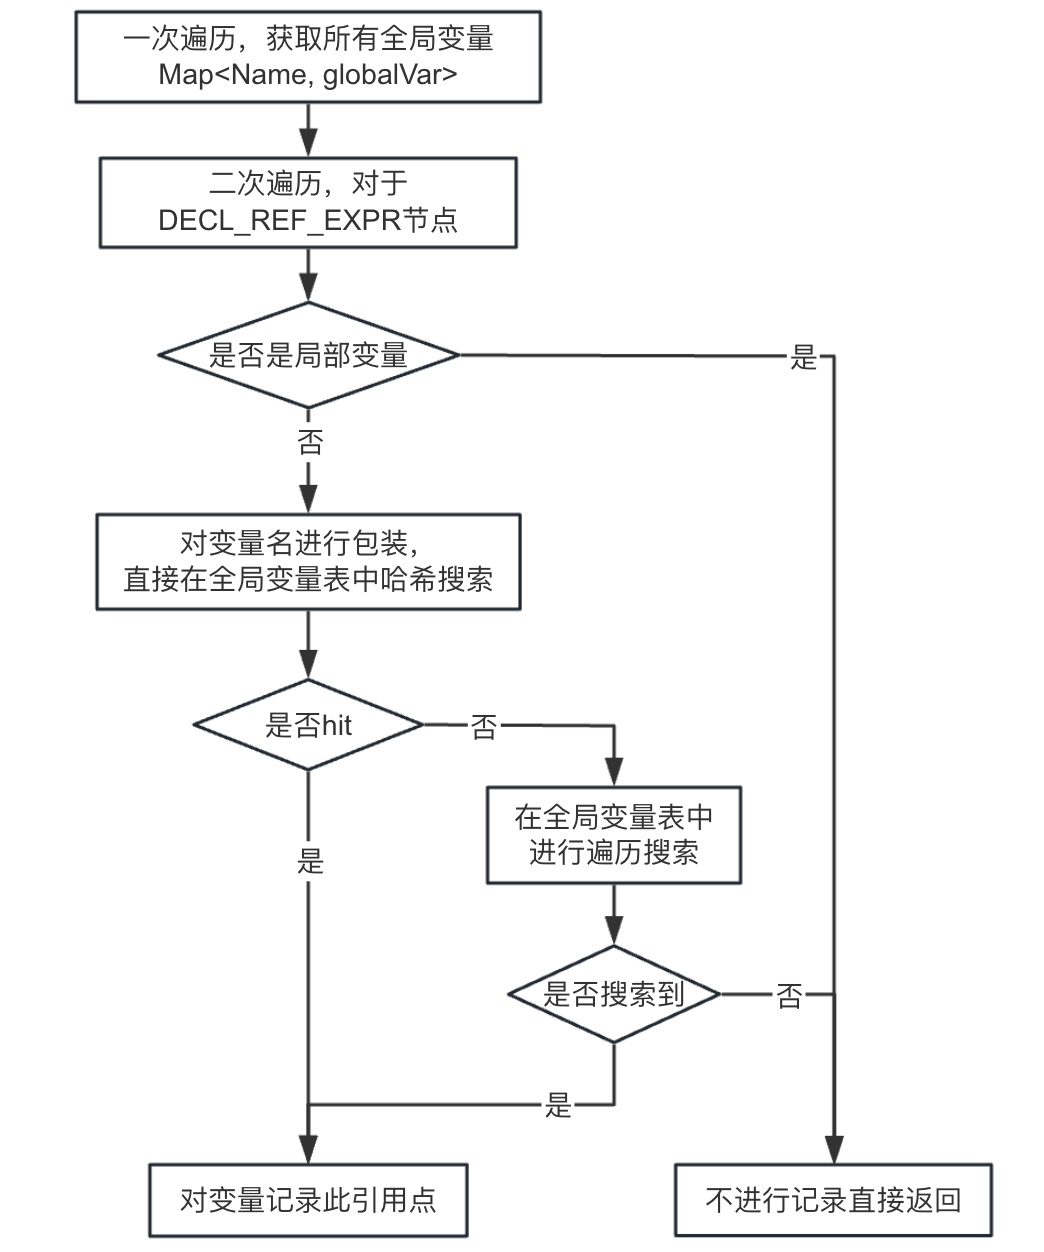
\includegraphics[width = 0.6\textwidth]{全局变量提取流程图}
\caption{示例代码对应的抽象语法树结构}
\end{figure}


分析结束后,将会获得每个全局变量的定义-引用链,对应于一个全局变量信息表,
包括项目代码中所有的全局变量和变量的引用点,除此之外还包括全局变量的类型、作
用域和所在文件等其他信息。

\section{基于方法特征的代码度量提取}

代码内聚度和代码耦合度是衡量软件设计质量的两个核心指标,它们直接反映了代
码质量。代码内聚度指的是模块(如函数、类或组件)内部元素之间的相关性。高内聚
度意味着模块内的所有元素都紧密地围绕着一个单一的、明确的功能,代码更容易理解
和维护[9]。代码的耦合性则描述了模块之间的相互依赖。低耦合度意味着模块之间的依
赖关系最小化,每个模块都可以独立地执行其功能,而不需要过多地依赖其他模块。低
耦合度的代码更容易测试和维护[10]。


基于方法摘要和全局变量信息表,我们计算如下代码度量,用于分析代码质量。


\subsection{基于内聚度缺乏度的内聚性分析}

LCOM(Lack of Cohesion in Methods)系列指标用于衡量模块的内聚度。本课题中
面向对象语言以类为研究范围进行计算内聚度,非面向对象的语言以文件为研究范围进
行计算,类中的成员属性对应文件中的全局变量,类中的成员方法对应文件中定义的方
法。LCOM 指标的核心思想是测量一个类中方法对实例变量(属性)的共享程度。不同
版本的 LCOM 有着不同的计算方法和含义。这里我们一共计算以下四个指标:


(1)LCOM1,含义是不引用相同字段的方法对数目[11]。

其中,P 是不共享实例变量的方法对的数量,Q 是共享实例变量的方法对的数量。
如果 LCOM1 的结果为负数,则被置为 0。
在计算时,对于每个文件首先构建方法耦合图(method coupling graph),将提取到
的方法作为图中节点,对方法两两进行判断,如果两个节点都引用相同的字段,则它们
之间用一条无向边连接,按如下公式计算,其中 n 是文件中的方法总数,e 是图中的实
际边数,即图中可能的最大边数减去实际的边数,得到的值即为 LCOM1

(2)LCOM2,含义是不引用相同字段方法对与引用相同字段方法对数之差[12]。
LCOM2相比于LCOM1,考虑到了类中所有方法和变量的相互作用,其计算公式是:
其中,�是类中属性的数量,��是访问属性�的方法数量。
在计算时,首先构建方法属性图(method-attribute graph),将提取到的方法和全局
变量作为图中节点。如果方法引用了变量,则有一条有向边从方法节点指向属性变量,
计算公式如下,

其中 n 为方法数,a 为变量数。假设 e 是图中的实际边数,得到的值即为 LCOM2。

(3)LCOM3,含义是以方法为顶点,两方法引用相同字段则有边构成的无向图的连通
分支数[12]。
LCOM3 是对 LCOM2 的进一步改进,其计算公式是:
其中,m 是类中方法的数量,a 是类中属性的数量,��是第 i 个方法访问的属性数
量,��是被第 i 个方法访问的属性数量。LCOM3 试图通过分析方法和属性之间的关系
来提供更细致的内聚度度量。

计算时的公式如下,基于上述计算出的 LCOM2 指标可以快速地计算出 LCOM3

(4)LCOM4,含义是以方法为顶点,两方法引用相同字段或有调用关系则有边构成无
向图的连通分支数[13]。
计算时,构建方法耦合图,节点是方法。如果两个节点都引用相同的字段,则它们
之间用一条无向边连接,除此之外,如果两个节点有调用关系,则也用一条无向边将它
们连接。根据深度搜索的方式,计算图中的连通分支数,得到的值即

\subsection{基于连通性的内聚性分析}
(1)TCC(Tight Class Cohesion)和 LCC(Loose Class Cohesion)是两种用于衡量类内
聚度的指标,它们主要关注于类中方法之间的连通关系。这两个指标的核心思想是通过
分析类中方法如何相互作用以及如何访问共同资源(如类级变量)来评估类的内聚度。
(1)TCC,含义是有关系方法对数/方法对总数[14]。
TCC 关注于类中方法之间的“直接连接”。如果两个方法直接共享访问同一个类级变
量,则认为这两个方法是直接连接的。计算时,对于每个文件首先构建方法耦合图,对
方法两两进行判断,如果两个节点都引用相同的字段,则它们之间用一条无向边连接,
按如下公式计算,其中 n 是文件中的方法总数,e 是图中的实际边数

(2)LCC,基于方法间接引用共同字段关系的传递闭包计算[14]。
LCC 除了考虑直接连接的方法对外,还包括了间接连接的方法对。如果两个方法不
是直接连接,但可以通过一系列的方法调用来连接,则认为它们是间接连接的。LCC 的
值基于类中直接或间接连接的方法对占所有可能方法对的比例来计算。因此,LCC 的值
通常不低于 TCC 的值,并且提供了一个更宽泛的类内聚度视角。
计算时,对于每个文件首先构建方法耦合图,对方法两两进行判断,如果两个节点
都引用相同的字段,则它们之间用一条无向边连接表示直接连接,如果方法之间有调用,
则也将方法进行连接,并连接当前节点和调用节点的所有邻居节点。按如下公式计算,
其中 n 是文件中的方法总数,e 是图中的直接连接边,lj ��푑�ǖ lj �怀是除直接连接边的边数。


\subsection{方法间耦合性分析}

耦合是软件结构中各模块之间相互连接的一种度量,根据耦合程度可以分为 6 种,
耦合度依次变低。


内容耦合是指一个模块可以直接访问另一个模块的内部数据,由于我们分析的是方
法粒度的耦合关系,而在方法之间并不存在此种情况,故不关注这种耦合关系。


公共耦合是指多个模块都访问同一个公共数据环境,公共数据环境例如全局数据结
构、内存公共覆盖区等。在提取到的全局变量表中,针对复杂类型的数据结构,如结构
体、数组结构等,它们的引用点所在的方法,两两之间都存在此种公共耦合关系。


外部耦合指多个模块访问同一个全局简单变量。与公共耦合类似,在提取的全局变
量表中,对于基本类型的全局变量的引用点所在的方法,两两之间都存在此种外部耦合
关系。


控制耦合指模块之间传递信息中包含用于控制模块内部的信息。在提取到的方法摘
要表中,遍历方法,如果该方法调用其他方法时,对应方法的参数列表中有变量决定了
被调用方法中的计算流程,则方法之间存在控制耦合关系。


标记耦合指通过参数表传递数据结构信息,调用时传递的是数据结构。在方法摘要
表中,我们提取了方法的参数列表,包括参数名和参数类型,根据参数类型,可以确定
参数表中是否包含复杂类型。除此之外,在方法的调用表中,我们也提取了方法调用的
函数,结合这两个信息,即可确定两个方法是否存在着标记耦合关系。


数据耦合指通过参数表传递简单数据。与标记耦合类似,根据参数类型可以确定参
数是否全部为基本类型,结合方法调用表,即可确定两个方法是否存在数据耦合。
\subsection{方法扇入扇出度量分析}

函数的扇入(Fan-in)和扇出(Fan-out)是软件工程中用于衡量函数复杂性和模块
间依赖关系的两个指标。


扇入是指调用某个函数的不同函数的数量。它表示了一个函数对其他函数的依赖程
度。扇入值较高的函数通常被认为是重要的或核心的,因为它们被多个其他函数依赖。
高扇入值可能意味着该函数执行了一个基础或共享的任务。


扇出是指某个函数直接调用的不同函数的数量。它表示了一个函数对其他函数的影
响程度。扇出值较高的函数可能更复杂,因为它们需要管理和协调更多的函数调用。高
扇出值可能意味着该函数具有较高的责任度,且可能更难以理解和维护。

\begin{figure}[h]
\centering
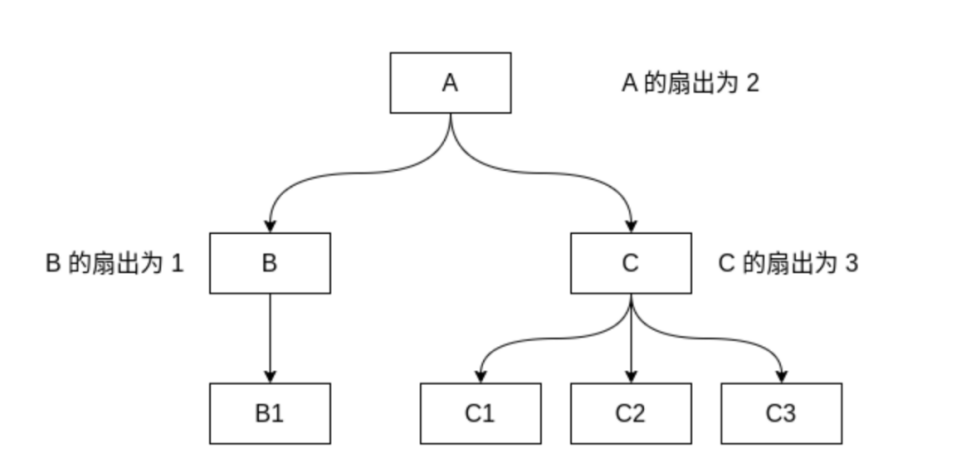
\includegraphics[width = 0.6\textwidth]{扇入扇出.png}
\caption{扇入扇出示例图}
\end{figure}

对于提取到的方法摘要表,遍历每一个方法,统计其调用方法的数量即可计算出该
方法的扇出值,再以该方法名在方法摘要表中搜索调用了该方法的方法,统计总数,得
到的值即为扇入值。

\section{本章小节}

%%%%%%%%%%%%%%%%%%%%%%%%%%%%%%%%%%%%%%%%%%%%%%%%%%%%%%%%%%%%%%%%%%%%%%%%%%%%%%%
\chapter{变更影响分析方法}
\section{引言}
方法之间的变更影响的类型可以分为以下三种类型:

(1)有直接调用关系
这种变更影响关系是显而易见的。比如方法 funcA 调用了方法 funcB,那么当 funcB
的方法签名有所变化时,调用它的方法必须对应地修改代码才能正常调用,否则会调用
不成功,甚至直接发生编译错误。

(2)共同调用另一个方法
如当 funcA 和 funcC 同时调用了方法 funcB 时,funcA 和 funcC 之间会有变更影响
关系。这种变更影响关系实际上是类型 1 的扩展,这种情况通常是 funcB 的更改引起了
funcA 和 funcC 的同时更改。

(3)逻辑上存在变更影响关系
这种变更影响关系中,方法之间虽然没有直接的调用关系,也不共同调用某个方法,
但它们的实现逻辑或者所操作的数据之间存在某种隐含的关联。这种关系可能是由于它
们共同维护某个数据的一致性、共享某些资源或者它们的输出和输入之间存在某种预期
的联系。因此,当其中一个方法发生变化时,可能会间接影响到其他方法的行为或结果,
即使这种影响在代码的静态结构中不直接可见。

\section{基于依赖关系闭包的变更影响分析}

在代码变更影响关系分析中,依赖关系传递闭包分析是一种用来预测代码变更可能
影响到的其他部分的技术[15]。这种方法依赖于对代码中各个元素之间依赖关系的深入
分析,通过这些依赖关系的传递来识别受影响的代码方法。这种变更影响关系是后续进
行模块化分析的基础。

首先识别直接依赖关系。包括函数调用、变量引用等。此前提取到的方法摘要表和
全局变量信息表已经包含了这种直接依赖关系。接下来将依赖关系表示为一个有向图,
其中节点代表代码中的元素,包括方法、全局变量,有向边代表依赖关系。这个依赖图
是分析代码变更影响的基础。对于依赖图中的每个节点,计算其传递闭包。传递闭包是
指从该节点出发,通过依赖关系可以直接或间接到达的所有节点的集合。这一步骤通过
图深度优先搜索来实现。

对于图中的所有方法节点进行变更影响分析,我们假设该节点有变更,计算传递闭
包后,得到的方法集合即为与当前方法有变更影响关系的方法。

以图 2-5 为例,在这个例子中,一共有 4 个方法,其中方法 funcA 调用了 funcB 和
funcD,funcB 调用了 funcC。在对 funcC 进行变更影响分析时,会直接影响到 funcB,
根据依赖关系闭包,会间接影响到 funcA。所以与 funcC 有变更影响关系的方法集合为
{funcB, funcA}。

\begin{figure}[h]
\centering
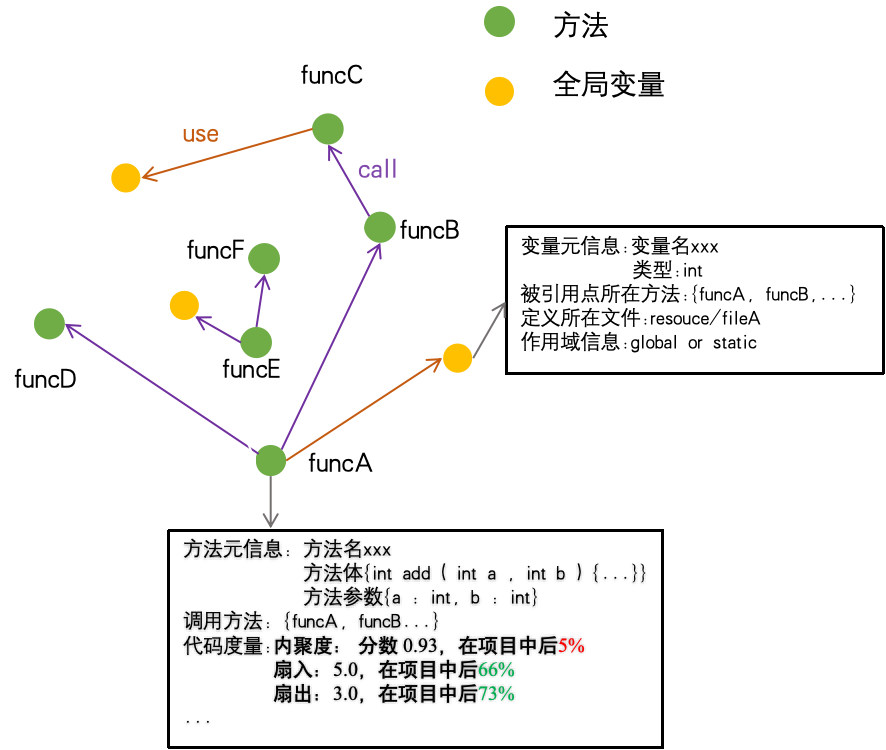
\includegraphics[width = 0.6\textwidth]{依赖关系示例.png}
\caption{依赖关系示例}
\end{figure}

\section{基于代码克隆的变更影响分析}
\subsection{代码分段及代码指纹提取}
\subsection{基于ClaSP算法的代码克隆检测方法}

\section{基于数据挖掘的变更影响分析}
\subsection{代码变更历史提取}
基于依赖关系闭包的方法可以识别方法之间浅层的变更影响关系,主要针对的是语
法和依赖关系层面,而无法抽取更深层的关系,因此设计了基于数据挖掘技术的变更影
响分析方法。本方法主要针对拥有代码变更历史记录的软件项目。其主要理论是认为在
代码变更历史中,频繁出现同时更改的方法对是存在着一定的变更影响关系的。这一过
程可以分为以下几个步骤:

这里为方便分析代码变更历史,主要分析对象为 git 项目。首先是收集项目的代码
库及其变更历史记录。然后,提取项目中的所有提交(commit),每个提交可能包含多
个更改文件。对于标记为“修改”的文件,提取所有变化的代码行,并定位这些代码行在
源代码中的方法,进而提取该方法体。收集每个提交中所有变更的函数,形成一个与该
提交相关的变更函数列表。

\subsection{基于频繁模式挖掘的变更影响关系提取}

接下来,基于数据挖掘中的频繁模式挖掘理论,识别可能存在变更影响关系的函数
对。频繁模式指的是在数据集中经常一起出现的项目或特征组合,而频繁项集是频繁模
式的具体表现形式。频繁项集是指在数据集中经常同时出现的一组项,如果一个项集的
支持度(即该项集出现的记录占总记录数的比例)超过了预先定义的最小支持度阈值,
则认为该项集是频繁的。在分析提交时,针对一个方法 A,记录其在所有提交记录中出
现的次数为 N,而在这些提交中,统计其他出现的方法次数 M,如对方法 B,记录其出
现的次数为 M。如果 M/N 的值为设定的阈值= 1,则认为方法对(A,B)有变更影响
关系。换言之,这意味着每当 A 出现时,B 也必然出现,方法对(A, B)每次更改都
为同时更改。

遍历项目变更历史,抽取出有变更影响关系的方法对,认为它们之间存在着变更
影响关系

对收集到的数据进行分析,这里以真实项目中挖掘到的方法对为例,如图 2-6 中所
示,这个项目是 kafka 的一个 C/c++客户端。方法一的主要功能是在 Kafka 模拟环境中
按照一定的规则生成 Producer ID,而方法二的功能是检查一个 Producer ID 是否有效。
当涉及检查的逻辑时,往往需要考虑到它是如何被创建和分配的。在这个例子中需要确
保 ID 的创建逻辑与检查逻辑一致,才能确保检查是正确的。这个方法中,对于要检查
的 Producer ID,首先会判断事务 ID,然后再检查 epoch,逻辑与创建 ID 是形成对应的。
考虑修改的行为,如果对于 Producer ID 的创建和分配逻辑进行了修改,那么通常需
要同时修改 Producer ID 检查逻辑,以确保两者保持一致。否则,如果创建和分配逻辑
发生了变化,而检查逻辑没有相应地进行调整,就可能导致检查逻辑无法正确地验证新
生成的 Producer ID,从而引入错误和不一致性。

\begin{figure}[h]
\centering
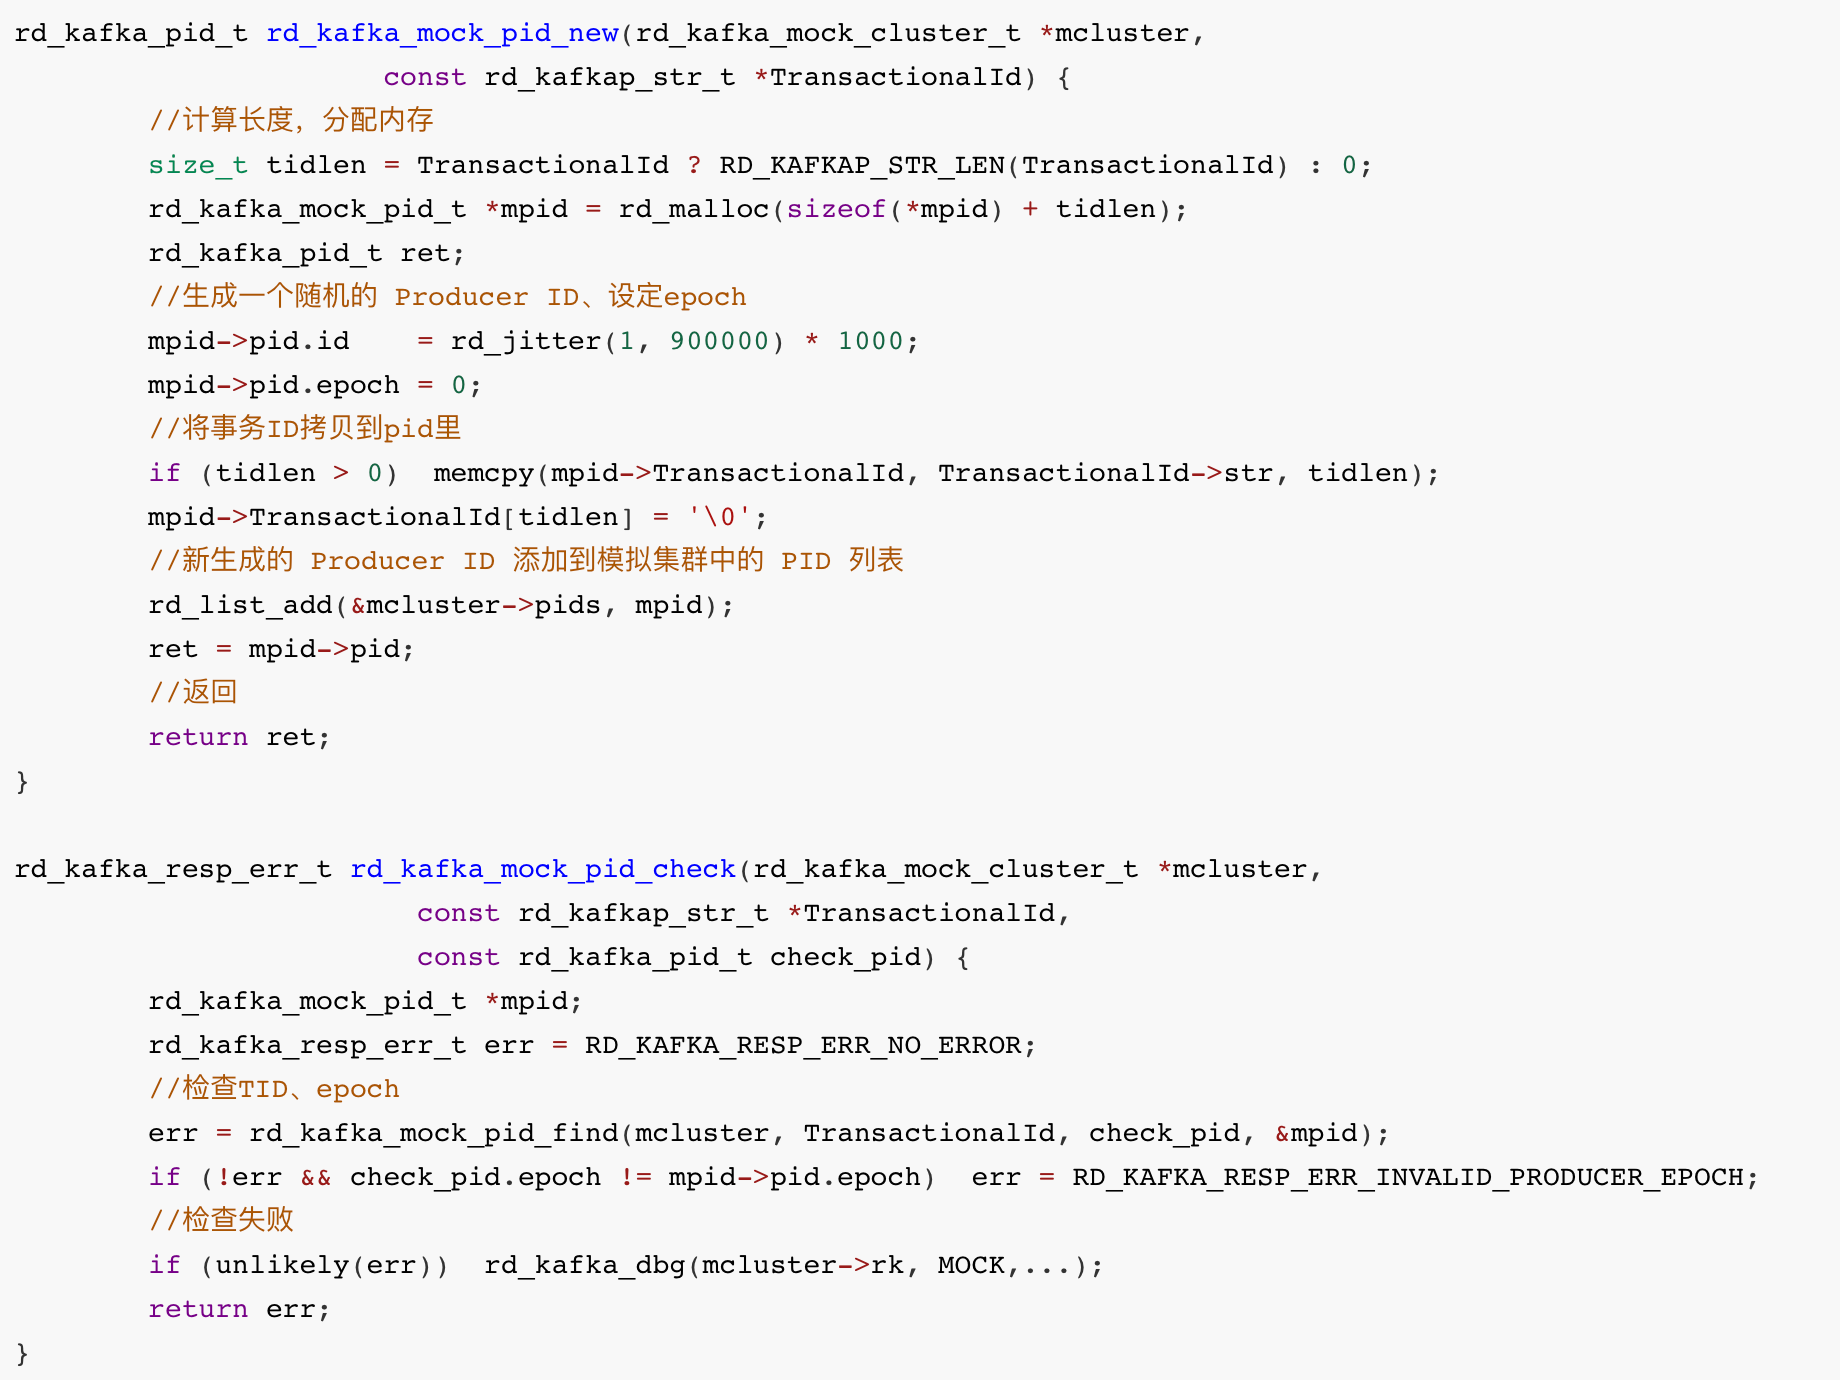
\includegraphics[width = 0.6\textwidth]{数据挖掘挖到的方法对.png}
\caption{逻辑上有变更影响关系的方法对示例}
\end{figure}


经过分析可以看出,通过数据挖掘方法得到的具有变更关系的方法对,是具有一定
的准确性的,并且可以弥补静态分析的不足。

\section{基于深度学习的变更影响分析}

当项目代码有丰富的变更历史时,可以根据数据挖掘的方式,抽取具有变更影响关
系的方法对,但是当只有项目源代码时,则只能根据静态分析的方式分析。本课题将数
据挖掘得到的数据作为数据集,训练深度学习模型,将模型用于对方法对的变更影响关
系预测,以弥补静态分析方法的不足。

\subsection{数据集的采集与预处理}

根据数据挖掘的变更影响关系分析的方法,可以提取到具有频繁同时更改的方法对,
将这种方法对作为数据集的正例进行收集,然后对方法进行随机取样,作为数据集的负
例收集。

这里我们主要以表 2-1 中的 github 项目为基础收集数据集。选择这几个项目的原因
是它们的收藏数均在千以上,说明这些项目在开源社区中有着一定的影响力,使用比较
广泛。除此之外,这些项目社区比较活跃,还在不断更新迭代过程中,所以能提供较为
丰富的变更历史,以供我们分析。

\subsection{基于codebert的变更影响预测}

在进行学习模型的训练时,考虑到对代码的理解性,采用 CodeBERT 作为核心的代
码表示学习模型。首先,将两个方法体分别输入到模型中,通过模型的处理,得到两个
函数体各自的嵌入表示,分别记为 s1 和 s2。接着将这两个向量表示进行拼接,形成合
并后的向量表示。此合并向量随后被送入一个由两层组成的多层感知机(MLP)中进行
进一步的处理。在这个过程中,模型通过学习,尝试捕捉函数体之间的深层次关系。最
终,将模型的输出与真实标签之间做交叉熵损失来进行优化,以此来调整模型的参数,
使模型能够更准确地理解和表示代码之间的关系。

实验结果如表 2-2 所示。实验使用的数据集总共 6000 对左右,按照训练、验证、测
试 集 为 6:2:2 , 分 别 训 练 了 codebert 系 列 的 两 个 网 络 CodeBERTa-small-v1 和
codebert-base-mlm,具体结果如下:

从总体上来看,两个模型的性能均表现出色,但深入分析召回率(recall)和精确率
(precision)时,可以发现两个模型各有所长。

CodeBERTa-small-v1 模型更加重视精确率,强调预测出的正例的真实性和准确性。
这意味着它在确保预测结果的准确性方面做得很好,但这种方法可能会导致一些正确的
情况被漏掉,即存在漏报的情况。由于"small"模型的规模较小,参数数量较少,这可能
会使得模型在训练过程中更容易发生过拟合现象。

另一方面,CodeBERT-base-mlm 模型更加注重召回率,致力于捕捉尽可能多的正样
本。这种策略虽然能够覆盖更多的正例,但在这个过程中,也可能会引入一些误报,即
将一些实际上是负例的情况错误地判定为正例。大型模型由于具备更强的泛化能力,通
常能够更好地适应新的数据集。因此,为了获得更好的泛化性能,它们通常会牺牲一定
的精确率。

\section{本章小节}

%%%%%%%%%%%%%%%%%%%%%%%%%%%%%%%%%%%%%%%%%%%%%%%%%%%%%%%%%%%%%%%%%%%%%%%%%%%%%%%


\chapter{代码审查图生成}
\section{引言}
对整个项目的分析结果将以代码审查图的方式展示给用户。其中图的节点是代码元
素,包括方法和全局变量,方法和方法以及方法和全局变量之间的关系将以边的形式进
行展示。

\section{基于方法功能标签的方法聚类}
\subsection{基于大语言模型的方法功能标签生成}
\subsection{基于功能标签的方法聚类}

\section{代码审查图}
\subsection{代码审查图构建}
\subsection{代码审查图可视化}

图形可视化方案基于开源项目 G6,构建并展示最终的代码审查图。G6 是一个图形
可视化引擎,它提供了绘制、布局、分析、交互、动画等全方位的图形可视化基础功能。
在图形的节点与边被计算出后,将这些数据以 JSON 格式组织起来,这样可以让 G6 加
载这些远程数据源进行展示,同时也实现了计算逻辑与图形可视化的有效分离。


如图 2-8 所示,目前实现了节点的分类、设置节点属性,以及边的分类、设置边信
息等关键功能。为了提升交互体验,还增加了鼠标悬停时即可查看节点或边信息的便捷
功能。

\section{本章小节}



% Local Variables:
% TeX-master: "../main"
% TeX-engine: xetex
% End:
